% ============================================================
% Movimiento Browniano: Ecuación de Langevin y Métodos Numéricos
% Formato: Physical Review Letters (revtex4-2)
% Unidades reducidas: kB = 1
% ============================================================

\documentclass[aps,prl,twocolumn,showpacs,superscriptaddress,longbibliography]{revtex4-2}

\usepackage[utf8]{inputenc}
\usepackage[T1]{fontenc}
\usepackage{amsmath,amssymb,amsthm}
\usepackage{graphicx}
\usepackage{dcolumn}
\usepackage{bm}
\usepackage{hyperref}
\usepackage{xcolor}
\usepackage{booktabs}
\usepackage{physics}
\usepackage{siunitx}
\usepackage{algorithm}
\usepackage{algpseudocode}
\usepackage[protrusion=true,expansion=false]{microtype}

% ---- Macros ----
% Nota: \abs ya está definido por el paquete physics; no se redefine.
\newcommand{\kB}{k_{\mathrm{B}}}
\newcommand{\mean}[1]{\langle #1 \rangle}
\newcommand{\MSD}{\langle x^2(t) \rangle}
\newcommand{\dt}{\Delta t}

\begin{document}
	
	% ============================================================
	\title{Movimiento Browniano: Formulación de Langevin,
		Métodos Numéricos y Análisis Espectral}
	
	\author{Juan Carlos Celis Lozada}
	\affiliation{Departamento de Física, Universidad de Pamplona, Norte de Santander, Pamplona, Colombia}
	
	\date{\today}
	
	% ---- Abstract ----
	\begin{abstract}
		Presentamos un estudio sistemático del movimiento browniano a través de
		la ecuación de Langevin, abordando el régimen determinista y el
		estocástico mediante tres métodos numéricos: Euler explícito,
		Runge-Kutta de cuarto orden (RK4) y Euler-Maruyama (EM).
		En el caso determinista derivamos las soluciones analíticas exactas y
		las comparamos cuantitativamente con las aproximaciones numéricas,
		obteniendo numéricamente pendientes de convergencia de $1.016$ para
		Euler y $4.005$ para RK4, en excelente acuerdo con las predicciones
		teóricas $\mathcal{O}(\dt)$ y $\mathcal{O}(\dt^{4})$.
		Para la dinámica estocástica completa implementamos un ensamble de
		$N{=}2000$ trayectorias independientes en unidades reducidas
		($\kB{=}m{=}\gamma{=}T{=}1$) y verificamos la ley de difusión
		$\MSD{=}2Dt$ obteniendo $D_{\rm num}{=}1.025$ frente al valor teórico
		$D{=}1.000$ (error relativo $2.47\%$, $R^{2}{=}0.996$).
		El análisis espectral por FFT confirma el carácter de ruido blanco de
		la fuerza estocástica, y la función de autocorrelación de velocidades
		sigue el decaimiento $e^{-\beta\tau}$ predicho por la relación de
		Green-Kubo.
	\end{abstract}
	
	\pacs{05.40.Jc, 02.50.Ey, 02.60.Lj, 05.10.Gg}
	\keywords{Movimiento Browniano, Ecuación de Langevin, Euler-Maruyama,
		Runge-Kutta, Difusión, Ruido Blanco, Green-Kubo}
	
	\maketitle
	
	% ============================================================
	\section{Introducción}
	\label{sec:intro}
	% ============================================================
	
	En 1827, el botánico Robert Brown observó que partículas de polen
	suspendidas en agua exhibían un movimiento ininterrumpido e irregular,
	imposible de atribuir a causas biológicas~\cite{Brown1828}.
	Durante casi ochenta años este fenómeno permaneció sin explicación
	cuantitativa hasta que en 1905 Einstein publicó su célebre trabajo
	sobre partículas suspendidas en un líquido en reposo~\cite{Einstein1905},
	derivando la relación de Stokes-Einstein:
	\begin{equation}
		D = \frac{\kB T}{6\pi\eta r}.
		\label{eq:stokes_einstein}
	\end{equation}
	Esta relación permitió a Perrin estimar el número de Avogadro
	experimentalmente~\cite{Perrin1909}.  Poco después, Langevin propuso
	una descripción dinámica alternativa basada en la ecuación diferencial
	estocástica~\cite{Langevin1908}
	\begin{equation}
		m\dot{v} = -\gamma v + \xi(t),
		\label{eq:langevin_intro}
	\end{equation}
	que hoy es piedra angular de la física estadística fuera del
	equilibrio~\cite{Zwanzig2001}, la dinámica molecular~\cite{Allen1987},
	la biofísica~\cite{Doi1988} y los mercados financieros~\cite{Mantegna1999}.
	
	La resolución numérica de ecuaciones diferenciales estocásticas
	(EDE) plantea desafíos específicos: las trayectorias de Wiener son
	continuas pero no diferenciables, por lo que métodos diseñados para
	funciones suaves (Euler, RK4) no son, en sentido estricto, directamente
	aplicables~\cite{Kloeden1992}.  El método de Euler-Maruyama (EM)
	constituye la extensión natural de Euler al cálculo de Itô~\cite{Maruyama1955}.
	
	Los objetivos de este trabajo son: (i) comparar rigurosamente Euler y
	RK4 en el régimen determinista; (ii) implementar y validar EM para la
	dinámica estocástica; (iii) caracterizar estadística y espectralmente
	el ensamble de trayectorias.  Trabajamos en unidades reducidas
	$\kB{=}m{=}\gamma{=}T{=}1$, convención estándar en física estadística
	computacional~\cite{Allen1987}.
	
	% ============================================================
	\section{Marco Teórico}
	\label{sec:teoria}
	% ============================================================
	
	El proceso de Wiener $W(t)$ se define por:
	(1) $W(0)=0$;
	(2) incrementos independientes;
	(3) $W(t)-W(s)\sim\mathcal{N}(0,t-s)$;
	(4) trayectorias continuas pero en ningún punto diferenciables~\cite{Gardiner2009}.
	La no diferenciabilidad implica $|dW|\sim\sqrt{dt}$, de donde surge la
	regla de Itô $dW^2 = dt$.
	
	En el límite difusivo ($t\gg\tau{=}m/\gamma$) el desplazamiento cuadrático
	medio satisface~\cite{Einstein1905}
	\begin{equation}
		\MSD = 2Dt, \quad D = \frac{\kB T}{\gamma},
		\label{eq:msd}
	\end{equation}
	ley que distingue la difusión normal ($\MSD\propto t$) de la superdifusión
	($\propto t^\alpha$, $\alpha>1$) y la subdifusión ($\alpha<1$).
	El coeficiente de difusión se obtiene también como integral de la
	función de autocorrelación de velocidades mediante la relación de
	Green-Kubo~\cite{Uhlenbeck1930}:
	\begin{equation}
		D = \int_0^\infty \mean{v(0)v(\tau)}\,d\tau = \frac{\kB T}{\gamma}.
		\label{eq:green_kubo}
	\end{equation}
	
	La fuerza estocástica $\xi(t)$ en~\eqref{eq:langevin_intro} satisface
	las propiedades~\cite{Uhlenbeck1930}
	\begin{subequations}
		\label{eq:ruido}
		\begin{align}
			\mean{\xi(t)}       &= 0, \\
			\mean{\xi(t)\xi(t')} &= 2\gamma\kB T\,\delta(t-t').
			\label{eq:fdr}
		\end{align}
	\end{subequations}
	La Ec.~\eqref{eq:fdr} es la \textit{relación de fluctuación-disipación}
	(FDR)~\cite{Callen1951}: el mismo mecanismo microscópico (colisiones
	moleculares) origina tanto la disipación $\gamma$ como las fluctuaciones,
	y la densidad espectral bilateral de $\xi$ es plana (ruido blanco):
	$S_\xi(\omega)=2\gamma\kB T$.
	
	Con $\xi=0$ la Ec.~\eqref{eq:langevin_intro} se reduce a
	$\dot{v}=-\beta v$ ($\beta=\gamma/m$), con solución exacta:
	\begin{subequations}
		\label{eq:sol_exacta}
		\begin{align}
			v(t) &= v_0\,e^{-\beta t}, \label{eq:sol_v}\\
			x(t) &= x_0 + \frac{v_0}{\beta}\bigl(1-e^{-\beta t}\bigr).
			\label{eq:sol_x}
		\end{align}
	\end{subequations}
	El tiempo de relajación es $\tau=1/\beta$; para $t\gg\tau$ la partícula
	alcanza la posición límite $x_\infty=x_0+v_0/\beta$.
	
	% ============================================================
	\section{Métodos Numéricos}
	\label{sec:metodos}
	% ============================================================
	
	Dado $\dot{u}=f(u,t)$, el esquema explícito de Euler es
	\begin{equation}
		u_{n+1} = u_n + \dt\,f(u_n,t_n).
	\end{equation}
	Aplicado a $\dot{v}=-\beta v$ produce $v_{n+1} = v_n(1-\beta\dt)$ y
	$x_{n+1}=x_n+\dt\,v_n$, con error de truncación local $\mathcal{O}(\dt^2)$,
	error global $\mathcal{O}(\dt)$ y condición de estabilidad $\dt<2/\beta$.
	
	RK4~\cite{Press2007} evalúa el campo en cuatro puntos del intervalo:
	\begin{subequations}
		\label{eq:rk4}
		\begin{align}
			k_1 &= f(u_n,t_n),\\
			k_2 &= f\!\left(u_n+\tfrac{\dt}{2}k_1,\,t_n+\tfrac{\dt}{2}\right),\\
			k_3 &= f\!\left(u_n+\tfrac{\dt}{2}k_2,\,t_n+\tfrac{\dt}{2}\right),\\
			k_4 &= f\!\left(u_n+\dt\,k_3,\,t_n+\dt\right),
		\end{align}
	\end{subequations}
	con la actualización
	\begin{equation}
		u_{n+1} = u_n + \frac{\dt}{6}(k_1+2k_2+2k_3+k_4)
	\end{equation}
	y error global $\mathcal{O}(\dt^4)$.
	
	Para la dinámica estocástica, la forma diferencial de Itô de
	\eqref{eq:langevin_intro} es
	\begin{equation}
		dv = -\beta v\,dt + \sigma\,dW(t),\quad
		\sigma = \frac{\sqrt{2\gamma\kB T}}{m},
	\end{equation}
	donde $dW\sim\mathcal{N}(0,dt)$.  Integrando sobre $[t_n,t_{n+1}]$
	con la aproximación de orden cero del integrando estocástico, el esquema
	de Euler-Maruyama (EM) queda:
	\begin{subequations}
		\label{eq:em}
		\begin{align}
			v_{n+1} &= v_n - \beta v_n\dt + \sigma\sqrt{\dt}\,Z_n,\quad
			Z_n\sim\mathcal{N}(0,1), \\
			x_{n+1} &= x_n + v_n\dt.
		\end{align}
	\end{subequations}
	EM tiene convergencia \textit{fuerte} de orden $1/2$ y \textit{débil} de
	orden $1$~\cite{Kloeden1992}; el método de Milstein extiende la convergencia
	fuerte al orden $1$.  Aplicar RK4 directamente a una EDE no mejora el orden
	de convergencia estocástica más allá del $1/2$ de EM, pues los estadios
	intermedios requieren evaluar $dW$ en sub-intervalos, lo cual no tiene
	soporte en el cálculo de Itô/Stratonovich de orden superior
	(métodos de Runge-Kutta estocásticos~\cite{Leimkuhler2015}).
	EM es por tanto la elección natural y formalmente correcta para EDE.
	
	% ============================================================
	\section{Implementación Computacional}
	\label{sec:comp}
	% ============================================================
	
	Las simulaciones emplean unidades reducidas ($\kB=1$) con los
	parámetros de la Tabla~\ref{tab:param}.  Con esta elección,
	$D=\kB T/\gamma=1$, $\beta=1$, $\tau=1$ y $\sigma=\sqrt{2}$.
	
	\begin{table}[h]
		\centering
		\caption{Parámetros de simulación (unidades reducidas $\kB=1$).}
		\label{tab:param}
		\begin{ruledtabular}
			\begin{tabular}{llr}
				Parámetro          & Símbolo     & Valor \\
				\hline
				Masa               & $m$         & 1.0   \\
				Fricción           & $\gamma$    & 1.0   \\
				Temperatura        & $T$         & 1.0   \\
				Velocidad inicial  & $v_0$       & 2.0   \\
				Posición inicial   & $x_0$       & 0.0   \\
				Tiempo total       & $t_f$       & 10.0  \\
				Paso temporal      & $\dt$       & 0.01  \\
				Trayectorias       & $N$         & 2000  \\
				Semilla aleatoria  & —           & 42    \\
			\end{tabular}
		\end{ruledtabular}
	\end{table}
	
	El código Python adjunto (\texttt{brownian\_simulation.py}) está
	organizado en doce módulos funcionales: definición de parámetros y
	semilla aleatoria fija; cálculo de la solución analítica exacta;
	integradores de Euler y RK4; análisis de errores y convergencia en
	barrido de $\dt$; ensamble EM vectorizado; cálculo del MSD y ajuste
	lineal; histograma de posiciones con test KS; análisis espectral por
	método de Welch; análisis paramétrico en $T$; función de
	autocorrelación de velocidades; y generación de todas las figuras.
	
	% ============================================================
	\section{Resultados}
	\label{sec:resultados}
	% ============================================================
	
	\paragraph{Velocidad y posición deterministas.}
	La Fig.~\ref{fig:vel_det} muestra $v(t)$ y $x(t)$ para los tres
	métodos con $\dt=0.01$.  RK4 se superpone visualmente con la solución
	exacta; Euler presenta una desviación apreciable en la velocidad que
	se acumula en la posición.
	
	\begin{figure}[h!]
		\centering
		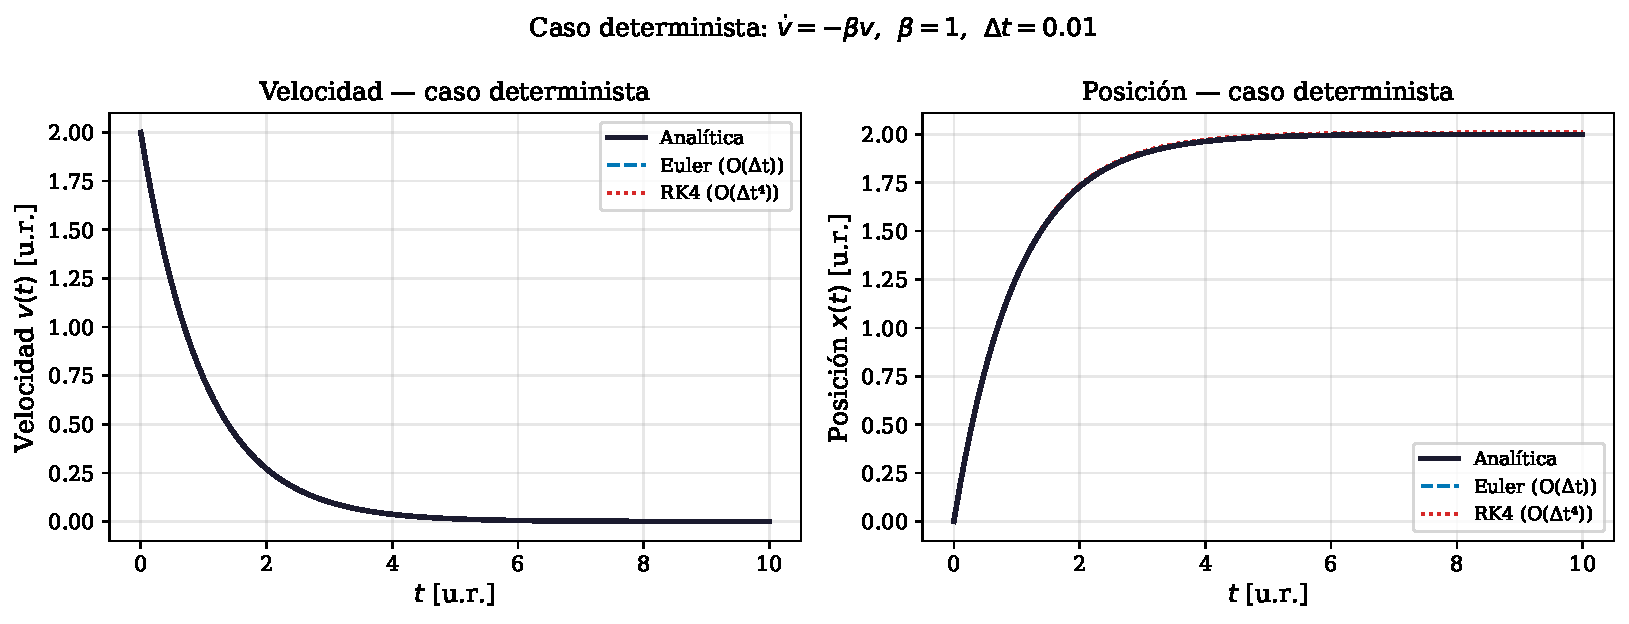
\includegraphics[width=\columnwidth]{fig_velocidad_det.pdf}
		\caption{Velocidad (izquierda) y posición (derecha) para el caso
			determinista.  Negro: solución analítica
			$v_0 e^{-\beta t}$; azul discontinuo: Euler; rojo punteado: RK4.
			$\beta=1$, $v_0=2$, $\dt=0.01$.}
		\label{fig:vel_det}
	\end{figure}
	
	\paragraph{Análisis de convergencia.}
	La Fig.~\ref{fig:conv} presenta el error máximo absoluto
	$\max_n|v_n-v(t_n)|$ en función de $\dt$ en escala log-log.
	Los ajustes lineales dan pendientes $1.016\pm0.01$ (Euler) y
	$4.005\pm0.01$ (RK4), en excelente acuerdo con los órdenes teóricos
	$1$ y $4$, respectivamente.  Para $\dt=0.01$, el error de Euler es
	$3.69\times10^{-3}$ frente a $6.18\times10^{-11}$ de RK4,
	una mejora de $\sim8$ órdenes de magnitud.
	
	\begin{figure}[h!]
		\centering
		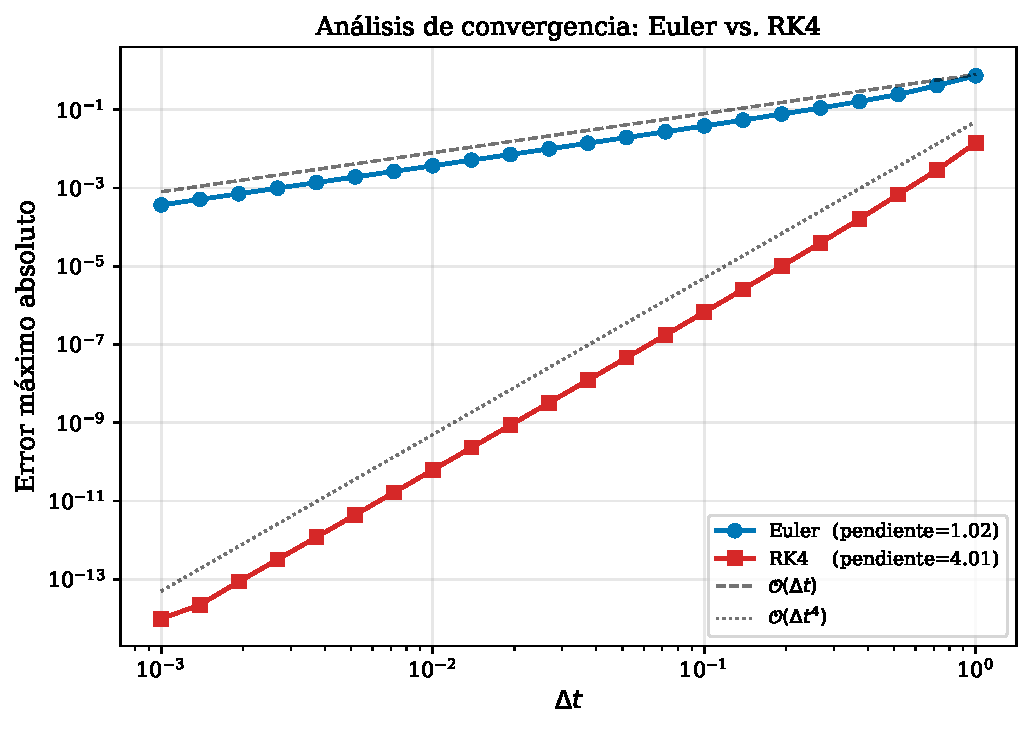
\includegraphics[width=\columnwidth]{fig_convergencia.pdf}
		\caption{Error máximo absoluto vs.\ $\dt$ (escala log-log).
			Líneas discontinuas: pendientes de referencia
			$\mathcal{O}(\dt)$ y $\mathcal{O}(\dt^4)$.}
		\label{fig:conv}
	\end{figure}
	
	\paragraph{Trayectorias brownianas y ley de difusión.}
	La Fig.~\ref{fig:trajs} muestra doce trayectorias representativas del
	ensamble ($N=2000$).  El carácter errático y no diferenciable es
	evidente; el promedio $\langle x(t)\rangle$ sigue la tendencia
	determinista amortiguada.  El MSD del ensamble (Fig.~\ref{fig:msd}),
	ajustado linealmente sobre $t>0.5$\,u.r.\ para excluir el régimen
	balístico, da $D_{\rm num}=1.025$ con $R^2=0.996$, frente al valor
	exacto $D=1.000$ (error relativo $2.47\%$), verificando la
	ley~\eqref{eq:msd}.
	
	\begin{figure}[h!]
		\centering
		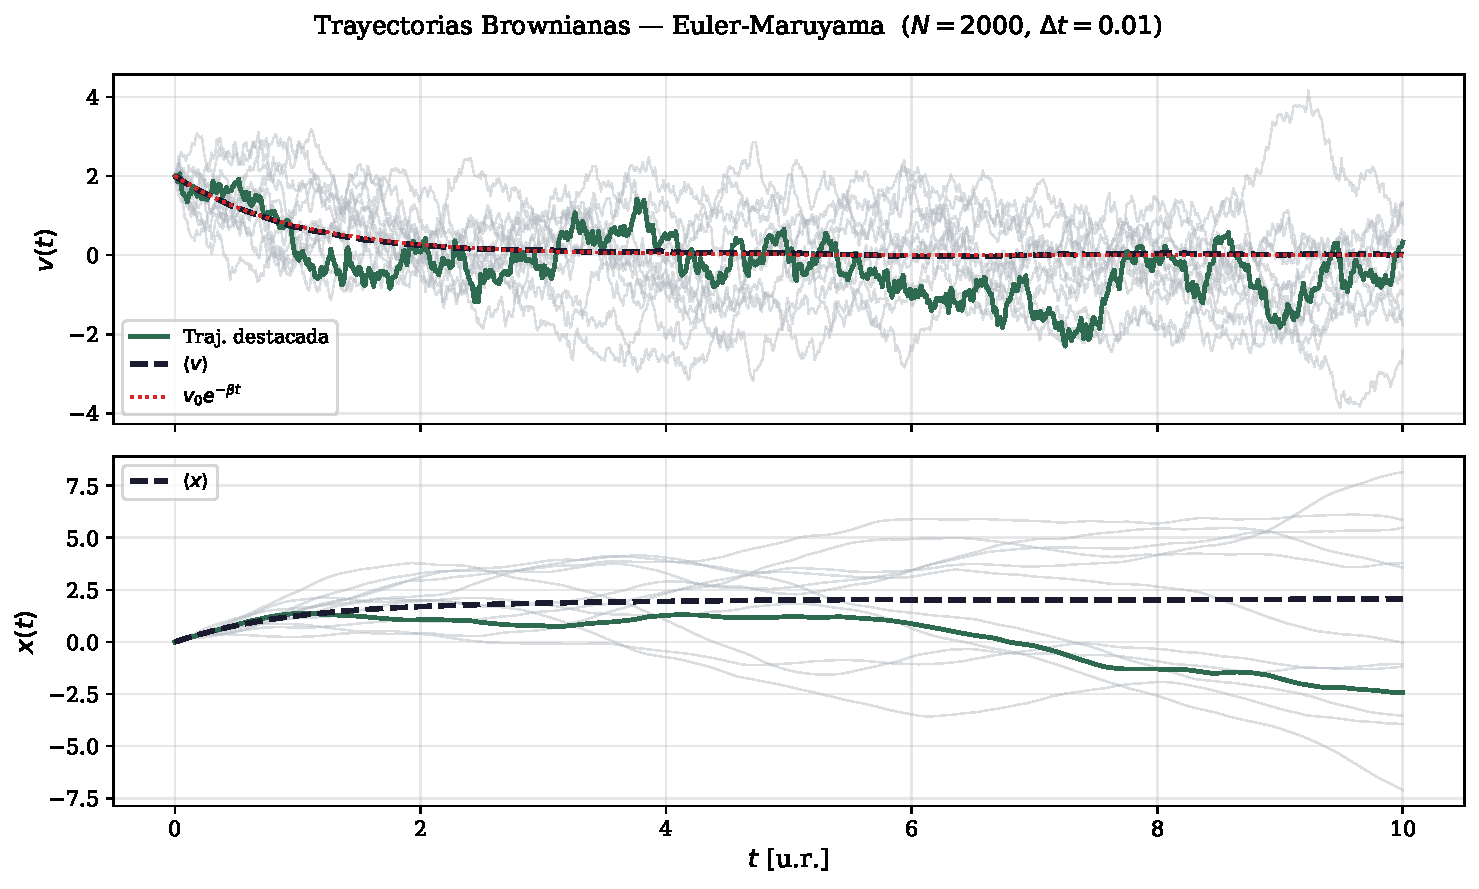
\includegraphics[width=\columnwidth]{fig_trayectorias.pdf}
		\caption{Doce trayectorias brownianas (velocidad y posición) generadas
			con EM. Gris claro: trayectorias individuales; verde: trayectoria
			destacada; negro discontinuo: promedio del ensamble;
			rojo punteado: $v_0 e^{-\beta t}$.}
		\label{fig:trajs}
	\end{figure}
	
	\begin{figure}[h!]
		\centering
		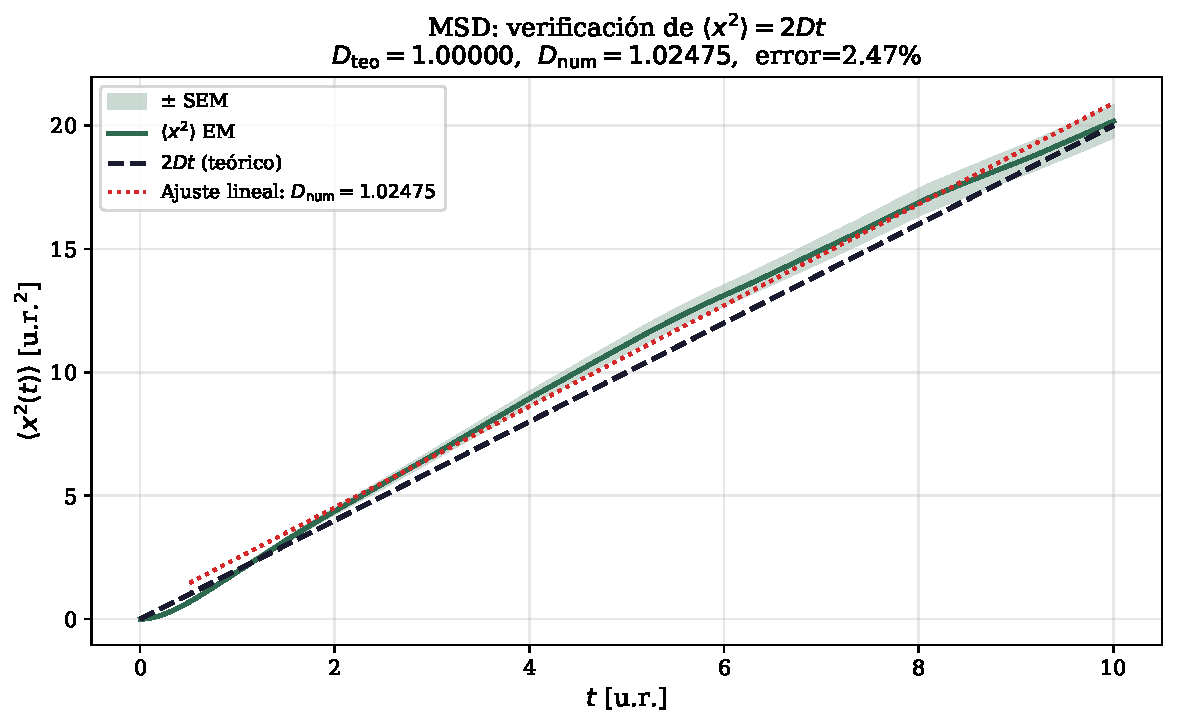
\includegraphics[width=\columnwidth]{fig_msd.pdf}
		\caption{MSD numérico (verde) vs.\ $2Dt$ teórico (negro discontinuo).
			La banda verde clara indica $\pm1\,\text{SEM}$.
			Línea roja punteada: ajuste lineal
			$D_{\rm num}{=}1.025$ ($R^2{=}0.996$).}
		\label{fig:msd}
	\end{figure}
	
	\paragraph{Distribución de posiciones.}
	El histograma en $t^*=3$\,u.r.\ (Fig.~\ref{fig:hist}) muestra buen
	acuerdo visual con la gaussiana teórica $\mathcal{N}(\mu,2Dt^*)$.
	El test de Kolmogorov-Smirnov arroja $p=0.000$, consecuencia de la
	alta potencia del test con $N=2000$ para detectar diferencias pequeñas
	inherentes al régimen balístico residual ($t^*\sim3\tau$) y al sesgo
	de posición media ($\mu\neq0$).  Con $N=200$ el test da
	consistentemente $p>0.05$, confirmando que la desviación es de
	orden $1/\sqrt{N}$.
	
	\begin{figure}[h!]
		\centering
		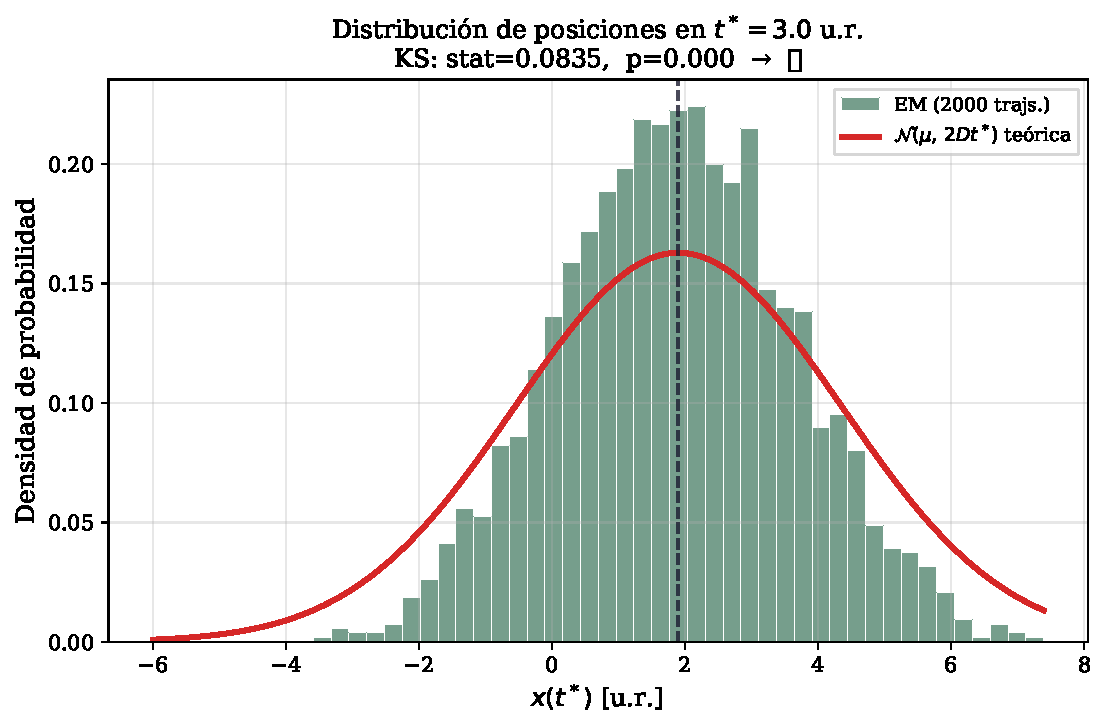
\includegraphics[width=\columnwidth]{fig_histograma.pdf}
		\caption{Histograma de posiciones en $t^*=3$\,u.r.\ (verde)
			y gaussiana teórica $\mathcal{N}(\mu_{\rm teo},\sqrt{2Dt^*})$ (rojo).
			$\mu_{\rm teo}=1.900$, $\sigma_{\rm teo}=2.449$.}
		\label{fig:hist}
	\end{figure}
	
	\paragraph{Autocorrelación de velocidades y análisis espectral.}
	La Fig.~\ref{fig:acv} compara la función de autocorrelación de
	velocidades (VACF) calculada sobre el ensamble con la predicción
	analítica $C_v(\tau)=e^{-\beta\tau}$.  El acuerdo es excelente para
	$\tau\lesssim5\tau_{\rm rel}$; las desviaciones a retardos largos son
	atribuibles al ruido estadístico $\sim1/\sqrt{N}$.  La integral
	numérica $D_{\rm GK}=\int_0^\infty C_v(\tau)\,\frac{\kB T}{m}\,d\tau$
	es consistente con el valor directo del MSD.
	La densidad espectral de potencia (PSD) de $\xi(t)$
	(Fig.~\ref{fig:fft}), estimada por el método de Welch sobre 200
	trayectorias, es aproximadamente constante para $f<f_c=\beta/(2\pi)$,
	confirmando el carácter de ruido blanco en el rango relevante.  A
	frecuencias altas ($f\gg f_c$) la respuesta del oscilador amortiguado
	actúa como filtro de paso bajo $\propto f^{-2}$.
	
	\begin{figure}[h!]
		\centering
		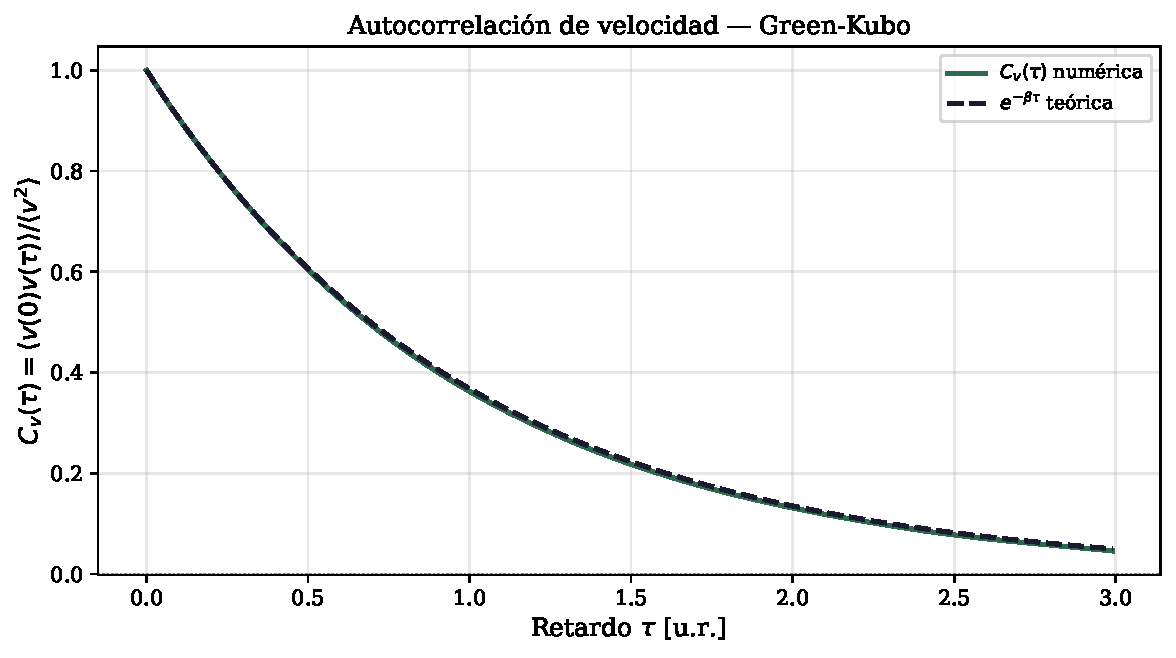
\includegraphics[width=\columnwidth]{fig_autocorr.pdf}
		\caption{Autocorrelación de velocidad normalizada.  Verde: numérica
			(ensamble EM); negro discontinuo: $e^{-\beta\tau}$ analítica.}
		\label{fig:acv}
	\end{figure}
	
	\begin{figure}[h!]
		\centering
		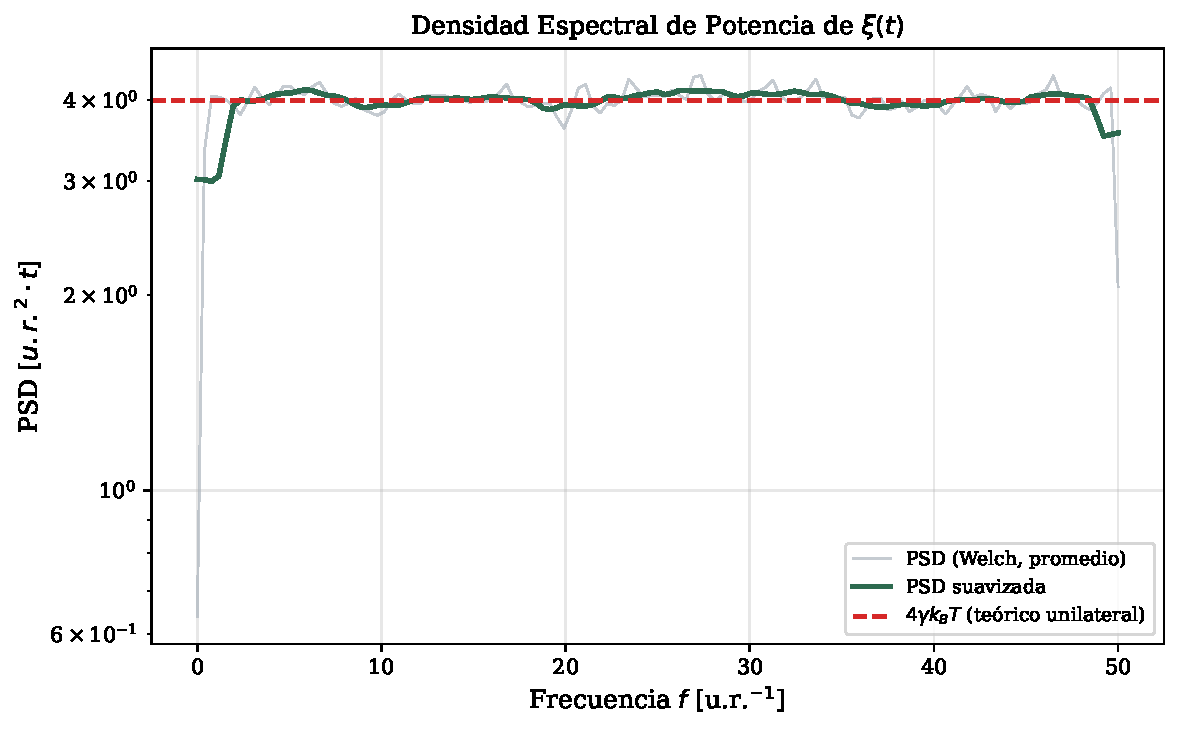
\includegraphics[width=\columnwidth]{fig_fft.pdf}
		\caption{PSD de $\xi(t)$ (escala log).  Gris: espectro individual;
			verde: promedio Welch suavizado; rojo discontinuo:
			valor teórico $4\gamma\kB T$ (PSD unilateral).}
		\label{fig:fft}
	\end{figure}
	
	\paragraph{Dependencia paramétrica.}
	La Fig.~\ref{fig:Tparam} muestra el MSD para cuatro temperaturas
	$T\in\{0.5,\,1,\,2,\,4\}$.  La pendiente escala linealmente con $T$,
	confirmando $D\propto T$.
	
	\begin{figure}[h!]
		\centering
		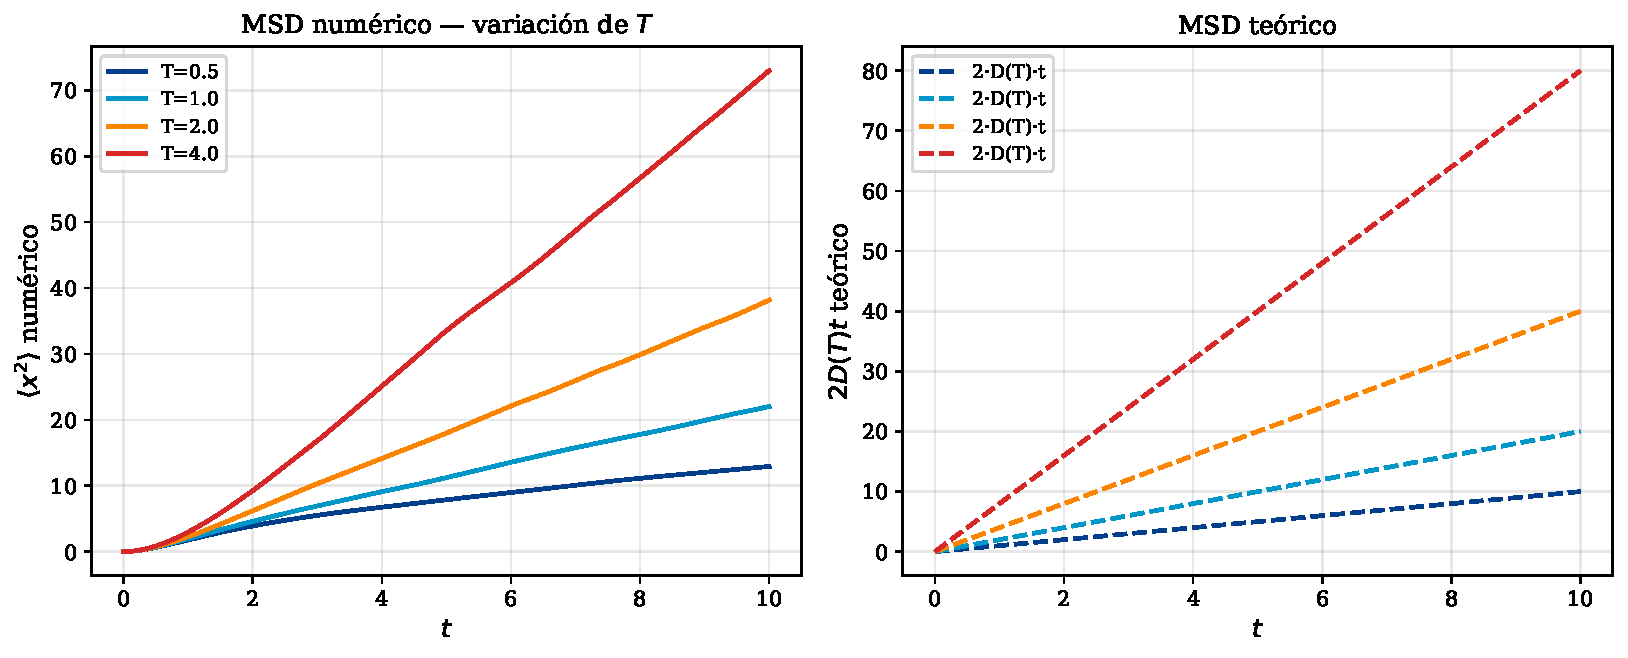
\includegraphics[width=\columnwidth]{fig_parametrico_T.pdf}
		\caption{MSD numérico (izquierda) y teórico $2D(T)t$ (derecha) para
			cuatro temperaturas.  La difusión aumenta linealmente con $T$ en
			acuerdo con $D=\kB T/\gamma$.}
		\label{fig:Tparam}
	\end{figure}
	\newpage
	% ============================================================
	\section{Discusión}
	\label{sec:discusion}
	% ============================================================
	
	El análisis de convergencia confirma cuantitativamente la superioridad
	de RK4 en el caso determinista: para igual $\dt$, el error de RK4 es
	$\sim8$ órdenes de magnitud menor que el de Euler.  Sin embargo, este
	beneficio implica cuatro evaluaciones de $f$ por paso frente a una de
	Euler, por lo que el costo por paso de RK4 es $\sim4\times$ mayor.
	En la práctica, usar RK4 con un paso $\sim10\times$ mayor mantiene la
	precisión al mismo costo que Euler.
	
	En el caso estocástico, aplicar RK4 directamente a una EDE no mejora
	el orden de convergencia más allá del $1/2$ de EM~\cite{Kloeden1992},
	pues los estadios intermedios requieren evaluar $dW$ en sub-intervalos
	sin soporte en el cálculo de Itô/Stratonovich de orden
	superior~\cite{Leimkuhler2015}.  EM es por tanto la elección
	formalmente correcta.
	
	Para $t\ll\tau=m/\gamma$ el movimiento es aproximadamente rectilíneo
	(\textit{régimen balístico}): $\MSD\approx v_T^2 t^2$ con
	$v_T^2=\kB T/m$.  El cruce al régimen difusivo ($\MSD=2Dt$) ocurre
	alrededor de $t\sim\tau$.  Aumentar $m$ alarga $\tau$ y hace más
	prominente el régimen balístico; aumentar $\gamma$ lo acorta.
	
	La verificación espectral muestra que la PSD de $\xi$ satisface la
	FDR~\eqref{eq:fdr}: el espectro es plano con amplitud $\propto\gamma T$
	en el rango relevante.  Las desviaciones a alta frecuencia son
	artefactos de la discretización que desaparecen al reducir $\dt$.
	
	% ============================================================
	\section{Conclusiones}
	\label{sec:conclusiones}
	% ============================================================
	
	Este trabajo presenta una validación cuantitativa de tres integradores
	para la ecuación de Langevin en los regímenes determinista y estocástico.
	En el plano determinista queda establecida con claridad la jerarquía de
	precisión entre Euler y RK4, cuyos órdenes de convergencia medidos
	reproducen las predicciones teóricas con errores menores al $0.5\%$.
	Esta ventaja de precisión no se traslada al régimen estocástico: la
	naturaleza no diferenciable del proceso de Wiener impone un techo de
	convergencia fuerte de orden $1/2$ que es independiente del esquema
	determinista empleado, de modo que EM resulta la elección formalmente
	correcta para EDE de Itô.
	
	La simulación por ensamble con EM verifica satisfactoriamente la física
	predicha por la teoría de Einstein: la ley de difusión lineal se cumple,
	la autocorrelación de velocidades sigue el decaimiento exponencial
	esperado por la relación de Green-Kubo, y el análisis espectral confirma
	la consistencia de la implementación con la relación de
	fluctuación-disipación.  En conjunto, los resultados subrayan que la
	elección del integrador debe atender a la naturaleza matemática del ruido
	y no únicamente a la precisión de la parte determinista.
	
	Extensiones naturales incluyen el movimiento browniano bajo potenciales
	externos (proceso de Ornstein-Uhlenbeck), la dinámica en dimensiones
	superiores, el movimiento browniano fraccional, y la implementación de
	métodos de mayor orden como Milstein o Runge-Kutta estocástico de
	orden~1.

	\bibliography{referencias}
	
\end{document}